\documentclass{article}

\usepackage{arxiv}

\usepackage[utf8]{inputenc} % allow utf-8 input
\usepackage[T1]{fontenc}    % use 8-bit T1 fonts
\usepackage{lmodern}        % https://github.com/rstudio/rticles/issues/343
\usepackage{hyperref}       % hyperlinks
\usepackage{url}            % simple URL typesetting
\usepackage{booktabs}       % professional-quality tables
\usepackage{amsfonts}       % blackboard math symbols
\usepackage{nicefrac}       % compact symbols for 1/2, etc.
\usepackage{microtype}      % microtypography
\usepackage{graphicx}

\title{Assessing the influence of dopamine and mindfulness on the
formation of task-relevant eye-movement patterns}

\author{
    Kelly G. Garner
   \\
    School of Psychology \\
    University of New South Wales \\
  Sydney, NSW \\
  \texttt{\href{mailto:insert.unsw@here.edu.au}{\nolinkurl{insert.unsw@here.edu.au}}} \\
   \And
    Li-Ann Leow
   \\
    School of Psychology \\
    The University of Queensland \\
  St.~Lucia, QLD \\
  \texttt{} \\
   \And
    Aya Uchida
   \\
    School of Psychology \\
    The University of Queensland \\
  St.~Lucia, QLD \\
  \texttt{} \\
   \And
    Ole Jensen
   \\
    Center for Human Brain Health \\
    University of Birmingham \\
  Birmingham, UK \\
  \texttt{} \\
   \And
    Marta Garrido
   \\
    School of Psychological Sciences \\
    University of Melbourne \\
  Melbourne, VIC \\
  \texttt{} \\
   \And
    Paul E. Dux
   \\
    School of Psychology \\
    The University of Queensland \\
  St.~Lucia, QLD \\
  \texttt{} \\
  }


% tightlist command for lists without linebreak
\providecommand{\tightlist}{%
  \setlength{\itemsep}{0pt}\setlength{\parskip}{0pt}}



\begin{document}
\maketitle


\begin{abstract}
Enter the text of your abstract here.
\end{abstract}

\keywords{
    blah
   \and
    blee
   \and
    bloo
   \and
    these are optional and can be removed
  }

\begin{verbatim}
## Loading required package: Rcpp
\end{verbatim}

\begin{verbatim}
## Loading 'brms' package (version 2.18.0). Useful instructions
## can be found by typing help('brms'). A more detailed introduction
## to the package is available through vignette('brms_overview').
\end{verbatim}

\begin{verbatim}
## 
## Attaching package: 'brms'
\end{verbatim}

\begin{verbatim}
## The following object is masked from 'package:stats':
## 
##     ar
\end{verbatim}

\begin{verbatim}
## -- Attaching packages --------------------------------------- tidyverse 1.3.2 --
## v ggplot2 3.4.0     v purrr   1.0.1
## v tibble  3.1.8     v dplyr   1.1.0
## v tidyr   1.3.0     v stringr 1.5.0
## v readr   2.1.3     v forcats 1.0.0
## -- Conflicts ------------------------------------------ tidyverse_conflicts() --
## x dplyr::filter() masks stats::filter()
## x dplyr::lag()    masks stats::lag()
\end{verbatim}

\hypertarget{introduction}{%
\section{Introduction}\label{introduction}}

Here goes an introduction text

\hypertarget{methods}{%
\section{Methods}\label{methods}}

\label{sec:Methods}

\hypertarget{participants}{%
\subsection{Participants}\label{participants}}

A total of 40 participants (mean age: 24.5, sd: 5, 30 female, 10 male)
were recruited using the undergraduate and paid SONA pools administered
by the University of Queensland. All procedures were cleared by the
University of Queensland Human Research ethics committee
{[}2017/HE000847{]}, and were conducted in accordance with the National
Statement on Ethical Conduct in Human Research. Participants were over
18 years old, had no known neurological and psychiatric conditions
(assessed by self report), and no contraindications to Levodopa, as
assessed by the Levodopa safety screening questionnaire. Informed
consent was obtained at the start of the first session.

\hypertarget{procedure}{%
\subsection{Procedure}\label{procedure}}

Participants attended two sessions, spaced approximately 1 week apart.
After initial blood pressure and mood assessments, participants received
either placebo (vitamin C) or Levodopa (Madopar 125: 100 mg Levodopa and
25 mg Benserazide Hydrochloride), crushed and dispersed in orange juice,
now referred to as the `placebo' and `DA' sessions respectively. The
solution was prepared by an experimenter who did not administer the
remaining experimental procedures. This protocol was sufficient to
achieve double blinding in previous work
(\textbf{chowdhuryDopamineModulatesEpisodic2012?};
\textbf{chowdhuryDopamineRestoresReward2013?}). Participants then
completed the Five Facet Mindfulness Questionnaire
(\textbf{baerUsingSelfReportAssessment2006?}) and the Barratt
Impulsivity Scale {[}BIS;
(\textbf{pattonFactorStructureBarratt1995?}){]}, as trait impulsivity
scores are associated with midbrain dopamine D2/D3 receptor
availability. Around 30 minutes after drug administration, participants
completed a second blood pressure and mood rating assessment.
Participants then completed the practice stage of the task, so that the
experimental stage began approximately 40 minutes after drug ingestion,
within the window of peak plasma availability. At the end of the
session, participants completed the final blood pressure and mood rating
assessment and were asked whether they thought they had been given the
active or placebo drug.

\hypertarget{apparatus}{%
\subsection{Apparatus}\label{apparatus}}

The experimental task was run with custom code\footnote{\url{https://github.com/kel-github/variability-decision-making}},
written using Matlab 2012b (32 bit) and Psychtoolbox v3.0.14, on a
Windows 7 (64-bit) on a Dell Precision T1700 desktop computer, displayed
using a ASUS VG248 monitor. Gaze coordinates (x, y) were sampled at 120
Hz using a monitor-mounted iView Red-m infrared eye tracker
(SensoMotoric Instruments GmbH, Teltow, Germany). Participants were
seated from the monitor at an approximate viewing distance of 57 cm, and
positioned on a chin-rest for the duration of the task.

\hypertarget{experimental-task}{%
\subsection{Experimental Task}\label{experimental-task}}

Each trial began with a fixation dot presented centrally on a grey
screen {[}RGB: 200 200 200{]}. Participants were instructed to fixate on
the dot to begin a trial. After 1000 ms of continuous correct fixation
samples (within 100 pixels of fixation), a square was presented that
comprsed 18° of degree visual angle along each length. The square could
be one of four possible colours {[}RGBs: 87, 208, 169; 267, 145, 52;
167, 162, 229; 239, 91, 158{]}. After 1000 ms, a 4 x 4 grid of smaller
squares appeared within the larger square, in a darker version of the
background colour ({[}RGB{]}-50). Each square comprised 2.6° of visual
angle. Participants were instructed that the 4 x 4 grid represented
doors, and that they were to use their eyes to open the doors to find
where the target was hiding. Participants were also instructed that they
were to fixate on a single door to open it. When participants had
fixated on a single door for over 300 ms, the door either turned black
{[}RGB: 50, 50, 50{]}, to denote the absence of a target, or the target
was displayed and the trial was terminated. If the door had turned
black, it returned to its previous colour as soon as it was detected
that the participant had moved their eyes from the door. Targets were
animal images drawn randomly on each trial from a pool of 100 images
taken from the internet. The time at which the target was available to
be found varied from trial to trial, with the onset being drawn from a
uniform distribution between 500-2000 ms. Once the target was available
and the correct door selected, the target was displayed for 750 ms. Upon
termination of the trial, the grey screen and white fixation cross were
presented (see Fig \ref{fig:taskFig}A).

In each session, participants were shown two possible background and
door colour sets. Participants were instructed that each colour
represented a world, and that the animals had different places they
preferred to hide, depending on the world they were in. There were four
possible target locations within each world, or from here on, visual
context. For each visual context, 1 door from each quadrant was selected
as one of the 4 target locations where the targets could appear (see Fig
\ref{fig:taskFig}B), with the constraint that target locations could not
overlap between contexts. Thus each colour reflected a context in which
participants could establish a set of task-relevant eye-movements,
i.e.~towards the 4 possible target locations for that context. Note that
within each context, the target was equally likely to appear behind any
one of the 4 target doors (p=.25) and would never appear behind the
remaining doors (p=0). Colour-target location mappings were
counterbalanced across participants, as was the assignment of coloured
contexts to sessions. Participants completed 80 trials in each context.
Eye-movement calibration and validation was performed every 20 trials.
Participants were also shown the standard QWERTY keyboard and were
instructed that they could press `x' at any time to perform a new
calibration and validation if they felt that their eye-movements were no
longer being registered accurately; i.e.~if they were unable to open
doors even though they were selecting them.

\begin{figure}

{\centering 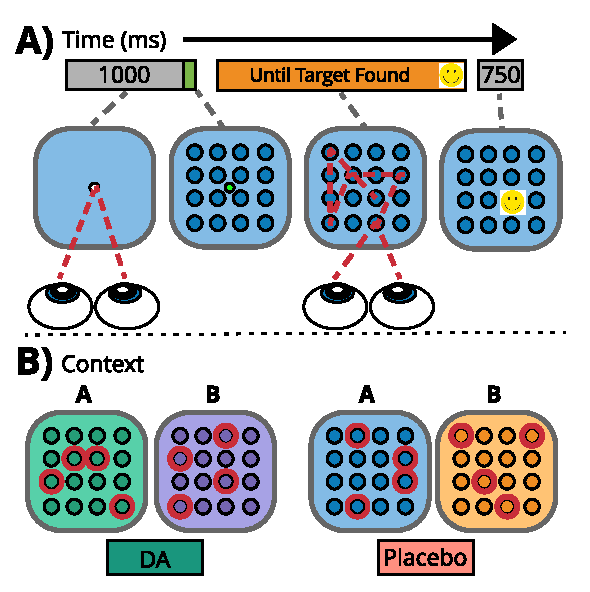
\includegraphics[width=0.7\linewidth]{../../images/DA_ExpTask} 

}

\caption{Experimental Task. A) A single trial where participants use their eyes to open doors to locate a target. B) Contexts and sessions: in each session, participants are exposed to two colour contexts each with 4 unique and equiprobable target locations. Colours and target locations were counterbalanced across participants and sessions. In each session, Levodopa (DA) or placebo is administered under double blind conditions.}\label{fig:taskfig}
\end{figure}

\hypertarget{statistical-approach}{%
\subsection{Statistical Approach}\label{statistical-approach}}

The analysis was designed to assess the learning of the target locations
given the context, the extent to which eye-movements became
stereotypical, and how both of these measures were modulated by the
dopamine and mindfulness factors. All custom analysis code is available
online\footnote{insert link}. The analysis was performed using R and
RStudio v2022.07.2 (\textbf{rstudiocitation?}), and can be reproduced in
the Neurodesk container environment
(\textbf{rentonNeurodeskAccessibleFlexible2022?}).

\hypertarget{data-cleaning}{%
\subsubsection{Data cleaning}\label{data-cleaning}}

Doors were marked as selected if participants gazed at them for a
duration of at least 300 ms. We assumed that a door could not be
selected twice consecutively, and collapsed any consecutive selections
into a single door selection. Last, as the final door selection of every
trial was fixed (i.e.~finding the target location ends the trial), we
removed the final selection from each trial for the sequence analysis
defined below. We excluded data from one participant whose total number
of door selections was greater than 3 standard deviations from the mean
across both sessions. The remaining 39 datasets were retained for all of
the analyses. Note that this is more inclusive than our pre-registered
plan for data exclusions\footnote{\url{https://osf.io/2y6pk}}. Based on
pilot data, we had planned to exclude participants who scored
\textless{} 65\% accuracy over the course of a session. Analysis of the
final sample suggested that this was too stringent, as this resulted in
the exclusion of 14 of 40 participants.

\hypertarget{accuracy}{%
\subsection{Accuracy}\label{accuracy}}

We first sought to determine the extent to which participants learned
the target locations, and then whether participants learned to select
the doors that were relevant given the current context. Door selections
were classified as target relevant (TR) for the current context (cc),
the other context from that session (oc), or neither (n). Data was then
grouped into blocks of 10 trials per context, and grouped across
contexts, resulting in 8 blocks of 20 trials. First, to determine
whether participants learned the target locations, regardless of
context, we computed accuracy as the number of times participants
selected a target door (referred to from now as accuracy {[}acc{]}),
relative to all door selections:

\[
acc = \frac{\sum{(TR_{cc}, TR_{oc})}}{\sum{(TR_{cc}, TR_{oc}, n)}}
\]

We assessed the influence of block, drug and mindfulness on accuracy
using a Bayesian mixed model approach. Accuracy was assumed to be drawn
from a binomial distribution (1=target door, 0 = non-target door). The
probability of drawing a target-door from the total number of door
selections made by a given participant was modelled logistic regression.
Note that as we use logistic regression, resulting regression parameter
values reflect changes to the log-odds of target door selections.

For this and following analyses, we found the model that best fit the
data, and made inference over the resulting parameters. We report the
95\% confidence intervals (CIs) of the parameter posteriors, and assume
we have detected a reliable effect when the 95\% CIs of the posterior do
not include zero. Models were fit using the BRMS
(\textbf{burknerBrmsPackageBayesian2017?}) interface for Stan
(\textbf{standevelopmentteamStanModelingLanguage?}) and RStan
(\textbf{standevelopmentteamRStanInterfaceStan2023?}). We used the
default weakly informative priors as specified in
(\textbf{burknerBrmsPackageBayesian2017?}). Specifically, fixed and
random effect \(\beta\) coefficients were given a flat prior, intercept
and standard deviations were assumed to be drawn from a student's \(t\)
distribution (df=1, location=0, scale=2.5), and the LKJ-correlation
prior with parameter \(\zeta\) \textgreater{} 0 was used for the
parameter covariance matrix. For each model, we checked for parameter
recovery using simulated data. Once fitted, we checked that the
residuals showed no signs of systematic error, that the chains had
converged, and that \(\hat{R}\) values were less than 1.01.

To eschew an overly large model space, and in line with our
pre-registration, we first fit models that contained each possible
combination of the block and drug regressors (and associated random
effects), and found the best model using leave-one-out (LOO) cross
validation (as implemented in
\textbf{vehtariPracticalBayesianModel2017?}). (Note that in the
pre-registration document we had proposed to compare models using the
deviance information criterion (DIC). As LOO is more robust than DIC to
influential observations, and is readily implemented for use with BRMS
model objects, we opted to use LOO instead of DIC). Upon identifying the
best model, we then added the mindfulness regressor using all possible
combinations, and once again selected the best model (as evidenced by
LOO). Last we controlled for trait impulsivity by adding BIS scores as a
main effect to the winning model. Note that in no cases did adding BIS
scores improve the model. We report the difference in the expected log
posterior density (ELPD) between the next best models and the winning
model, and the ratio of the ELPD difference to the standard error (SE)
of the difference (ELPD:SE), thus a negative ELPD difference reflects
preference for the winning model. The full set of model comparisons are
presented in the supplementary materials.

\hypertarget{contextual-accuracy}{%
\subsection{Contextual Accuracy}\label{contextual-accuracy}}

We next sought to understand whether dopamine modulates the ability of
participants to select the correct door, given the context. Therefore,
for each context, we computed the total number of cc door selections
(c-acc), and modelled the probability of attaining c-acc given the total
number of correct door selections:

\[
c\mathrm{-}acc = \frac{\sum{TR_{cc}}}{\sum{(TR_{cc}, TR_{oc})}}
\]

We then modelled this data using the Bayesian mixed effects approach
described above (Note that in the pre-registration document we had
suggested to include a regressor for context. Visual inspection of the
data showed that c-acc was highly comparable across contexts {[}see
supplemental figures{]}. We therefore opted to simplify the model space
and collapse over this factor).

\hypertarget{stereotypical-door-selections}{%
\subsection{Stereotypical door
selections}\label{stereotypical-door-selections}}

Next, we determined the extent to which door-selection patterns
increased in stereotypy over the course of the task, and whether
dopamine and mindfulness modulates the extent of stereotypy. Here we
define stereotypy as sets of door selections being deployed in the same
order, over trials (e.g. \textbf{desrochersHabitLearningNaive2015?}).
Therefore we wish to know whether, given the doors that a participant
chose to open over the trials of the experiment, does their data suggest
that they are selecting them in a more regularised manner as the
experiment progresses?

In order to characterise the extent to which door selections increased
in stereotypy, we reasoned that stereotypy should be evidenced by an
increase in the probability of a subset of door selection transitions,
at the expense of others. This stands in contrast to when making door
selections in an exploratory, or non-stereotyped way, where a greater
number of door transitions should show comparable probabilities.
Therefore, the transition probability matrices of individuals engaged in
more stereotypical door selections should show higher variance than
those who are not engaging in stereotypical door selections. We
therefore computed trial level transition probability matrices, and
computed the variance of each matrix. Variances were then collapsed
across context and trials to form a variance score for each participant,
session and block.

The resulting variance scores were subject to a comparable Bayesian
mixture modelling approach as described above with a few key
differences; the variance scores were assumed to be drawn from a skewed
normal distribution \(\mathcal{N}(\mu, \sigma, \alpha)\) whose mean
(\(\mu\)) was defined by the regression parameters (the distribution of
variance scores can be found in the supplemental materials). \(\sigma\)
was assumed to be drawn from a Student's t distribution (df=3,
location=0, scale=2.5), the skew parameter (\(\alpha\)) was assumed to
be drawn from a normal distribution \(\mathcal{N}(0,4)\). The remaining
priors for the intercept, beta-coefficients and parameter covariance
matrix were defined in the same manner as for the accuracy data models.
As the log-log plot of variances vs block suggested a power function,
analysis was performed on the logged data. This ensured that the
relationship between block and variance values was best described by a
straight line. Identification of the winning model proceeded as
described for the accuracy data above.

\hypertarget{blinding-analyses}{%
\subsection{Blinding analyses}\label{blinding-analyses}}

To determine whether awareness of the dopamine intervention could have
contributed to the findings, the probability of participant and
experimenter ratings were compared to the expected values assuming
chance guessing, using a binomial model. Blood-pressure and mood
measures were compared using {[}insert whether paired t-test or
Mann-Whitney U test{]}.

\hypertarget{results}{%
\section{Results}\label{results}}

HERE I INSERT THE BRIEFEST OVER VIEW OF ALL THE RESULTS

\hypertarget{accuracy-1}{%
\subsection{Accuracy}\label{accuracy-1}}

\hypertarget{model-selection}{%
\subsubsection{Model Selection}\label{model-selection}}

First we sought the model with the greatest predictive accuracy so that
we could make subsequent inference over the parameters. The model that
best accounted for the experimental factors contained main fixed effects
of block and drug, and random effects for block x drug. Although this
model was only closely preferred to the next most complex model that
contained a block x drug interaction (ELPD diff = -0.17, ELPD:SE =
-0.32), it was strongly preferred to all other models (min ELPD diff =
-674.10, ELPD:SE = -8.35). Adding mindfulness scores improved the
predictive accuracy of the model; the winning model contained an
additional main effect of mindfulness, two-way interactions with block
and with drug, and a 3-way block x drug x mindfulness interaction (ELPD
diff = -12.02, ELPD:SE = -1.88). Adding BIS scores did not improve the
predictive value of the model (ELPD diff = -0.16, ELPD:SE = -0.34). Note
that although we draw inferences over parameters from the winning model,
our inferences are the same as if we had used the more complex model
that includes the BIS scores.

\hypertarget{the-effect-of-drug-and-mindfulness-on-accuracy}{%
\subsubsection{The effect of drug and mindfulness on
accuracy}\label{the-effect-of-drug-and-mindfulness-on-accuracy}}

Having established the best model to account for the data, we next
determine the influence of DA and mindfulness on accuracy by making
inference over the resulting parameters. Accuracy data plotted by block
x drug session (DA va placebo) are shown in Fig \ref{fig:accfig}A.
Critically, the influence of drug on accuracy was impacted by
mindfulness scores. The drug x mindfulness parameter differed reliably
from zero (mean log odds = -0.11, 95\% CI{[}-0.16, -0.06{]}, see Fig
\ref{fig:accfig}E). To better understand this interaction, we computed a
score for each participant that reflected the mean accuracy change due
to the drug session (\(\mu\) acc{[}DA - P{]}). Note that a positive
score indicates that performance was better in the DA session relative
to placebo. Next we examined the relationship between drug-induced
accuracy changes and mindfulness scores. As can be seen in Fig
\ref{fig:accfig}B, there was a positive relationship between
drug-induced accuracy changes and mindfulness; participants scoring
higher for mindfulness showed higher accuracy for the DA relative to the
placebo session, for example, those scoring in the highest quartile
showed mean accuracy scores of 0.67 (95\%CI{[}0.65, 0.70{]}) during the
DA session, relative to mean accuracy scores of 0.62 (95\% CI{[}0.60,
0.63{]}) during the placebo session. Individuals scoring low on
mindfulness showed the opposite pattern (DA mean accuracy = 0.61, 95\%
CI{[}0.60, 0.63{]}, placebo mean accuracy = 0.68, 95\%CI{[}0.66,
0.69{]}), note that Fig \ref{fig:accfig}B shows the difference between
these accuracy scores). Thus the impact of DA on the establishment of
task-relevant eye-movements is dependent on the mindfulness state of the
individual.

Participants learned the target door locations over the course of the
sessions, accuracy reliably increased over blocks. Mean accuracy in
block 1 was 0.57 (95\% CI{[}0.55, 0.59{]}), relative to a block 8 mean
of 0.70 (95\% CI{[}0.68, 0.72{]}). The model showed that accuracy
increased by block with an average log odds of = 0.15, (95\% CI{[}0.09,
0.22, Fig \ref{fig:accfig}C). There was also the suggestion of a main
effect of the drug intervention (mean log odds = 0.04, 95\% CI{[}-0.001,
0.09, Fig \ref{fig:accfig}D), however, the impact of drug on accuracy is
presumably better explained by the drug x mindfulness interaction.

\begin{figure}

{\centering 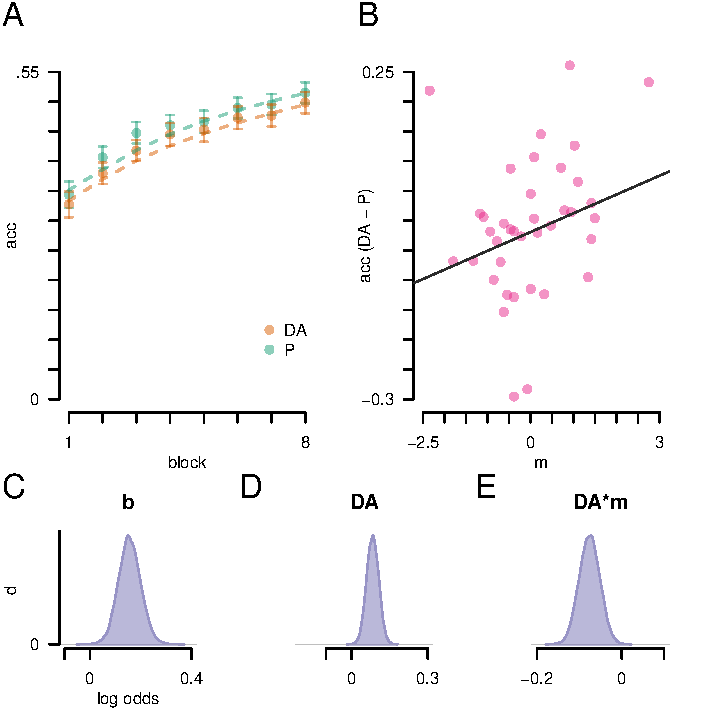
\includegraphics[width=0.7\linewidth]{../../images/acc_fig} 

}

\caption{The influence of dopamine and mindfulness on accuracy. A) Accuracy (acc) data by block and drug. Circles reflect observed average accuracy, dotted lines reflect the fit of the winning model. B) The association between trait mindfulness (x-axis) and the impact of drug on accuracy [DA-P]. The bottom row shows posterior densities (in log odds) estimated for C) the main effect of block (b), D) the main effect of DA, and E) the drug x mindfulness (m) interaction. DA = dopamine, P = placebo, d = density. Error bars reflect within-subject standard error of the mean [SE].}\label{fig:accfig}
\end{figure}

\hypertarget{contextual-accuracy-acc}{%
\subsection{Contextual accuracy (acc)}\label{contextual-accuracy-acc}}

\hypertarget{model-selection-1}{%
\subsubsection{Model Selection}\label{model-selection-1}}

The model that best accounted for the experimental factors contained
main fixed effects of block and drug, and random effects for block x
drug. Although this model was only closely preferred to the next most
complex model that contained a block x drug interaction (ELPD diff =
-0.66, ELPD:SE = -1.67), it was strongly preferred to all other models
(min ELPD diff = -553.79, ELPD:SE = -8.35). Adding mindfulness scores
improved the predictive accuracy of the model; the winning model
contained an additional main effect of mindfulness (ELPD diff = -0.13,
ELPD:SE = -0.12). Adding BIS scores did not improve the predictive value
of the model (ELPD diff = -0.02, ELPD:SE = -0.03). Note that although we
draw inferences over parameters from the winning model, our inferences
are the same as if we had used the more complex model that includes the
BIS scores.

\hypertarget{drug-and-not-mindfulness-impacts-contextual-accuracy}{%
\subsubsection{Drug, and not mindfulness, impacts contextual
accuracy}\label{drug-and-not-mindfulness-impacts-contextual-accuracy}}

Having established the best model to account for the data, we next
determined the influence of DA and mindfulness on accuracy by making
inference over the resulting model parameters (see Fig
\ref{fig:caccfig}. DA reduced contextual accuracy; accuracy was on
average 0.64 (95\% CI {[}0.63, 0.65{]}) for the DA session, and 0.66
(95\% CI {[}0.65, 0.68{]}) for the placebo session. The log-odds of
selecting a target door that was specific to the current context
increased by a mean log odds of 0.07 (95\% CI{[}0.01, 0.13, Fig
\ref{fig:caccfig}A\&B) for the placebo session, relative to the DA
session.

Participants learned to make contextually accurate door selections over
the course of the sessions; mean accuracy in block 1 was 0.59 (95\%
CI{[}0.58, 0.61{]}), relative to a block 8 mean of 0.69 (95\% CI{[}0.67,
0.71{]}). The model showed that contextual accuracy increased by a mean
log odds of 0.13 (95\% CI{[}0.07, 0.19) over each block (Fig
\ref{fig:caccfig}C). In contrast to the overall accuracy data,
mindfulness did not have a reliable impact on contextual accuracy (mean
log odds = 0.04, 95\% CI{[}-0.04, 0.15{]}).

\begin{figure}

{\centering 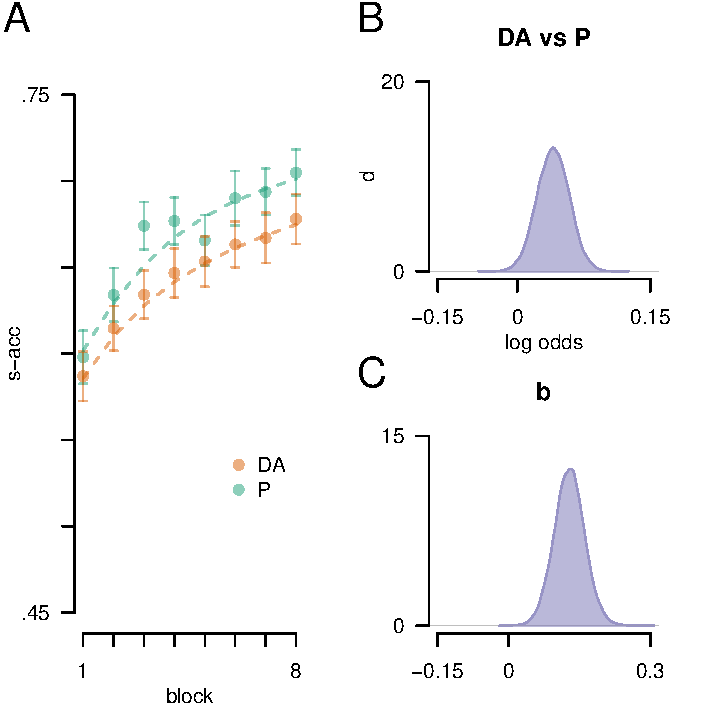
\includegraphics[width=0.7\linewidth]{../../images/cacc_fig} 

}

\caption{The influence of dopamine and mindfulness on contextual accuracy. A) Accuracy (acc) data by block and drug. Circles reflect observed average accuracy, dotted lines show the fit of the winning model. B) Estimated posterior density (in log odds) for the main effect of drug (DA vs P), D) same as in B, but for the main effect of block. DA = dopamine, P = placebo, b = block, d = density. Error bars reflect within-subject standard error of the mean [SE].}\label{fig:caccfig}
\end{figure}

\hypertarget{stereotypy-of-door-selections}{%
\subsection{Stereotypy of door
selections}\label{stereotypy-of-door-selections}}

\hypertarget{model-selection-2}{%
\subsubsection{Model Selection}\label{model-selection-2}}

The model that best accounted for the experimental factors contained
main fixed effects of block and drug, and random effects for block x
drug. Although this model was only closely preferred to the next most
complex model that contained a block x drug interaction (ELPD diff =
-0.26, ELPD:SE = -1.29), it was strongly preferred to all other models
(min ELPD diff = -130.14, ELPD:SE = -7.71). Adding mindfulness scores
improved the predictive accuracy of the model; the winning model
contained an additional main effect of mindfulness and a drug x
mindfulness interaction (ELPD diff = -3.15, ELPD:SE = -0.92). Adding BIS
scores did not improve the predictive accuracy of the model (ELPD diff =
-0.54, ELPD:SE = -1.41). Note that although we draw inferences over
parameters from the winning model, our inferences are the same as if we
had used the more complex model that includes the BIS scores.

\hypertarget{the-impact-of-drug-and-mindfulness-on-stereotypy}{%
\subsubsection{The impact of drug and mindfulness on
stereotypy}\label{the-impact-of-drug-and-mindfulness-on-stereotypy}}

In line with the notion that mindfulness and dopamine interact to impact
the formation of stereotypical door selections, we observed a reliable
drug x mindfulness interaction (mean \(\beta\) = 0.11, 95\% CI{[}0.02,
0.21, Fig \ref{fig:stereofig}). Participants scoring higher for
mindfulness showed lower stereotypy for the DA relative to the placebo
session, for example, those scoring in the highest quartile showed mean
log variance scores of -8.74 (95\%CI{[}-8.80, -8.68{]}) during the DA
session, relative to mean log variance scores of -8.68 (95\% CI{[}-8.74,
-8.62{]}) during the placebo session. Individuals scoring low on
mindfulness (lowest quartile) showed the opposite pattern (DA mean
accuracy = -8.69, 95\% CI{[}-8.75, -8.63{]}, placebo mean accuracy =
-8.72, 95\%CI{[}-8.78, -8.66{]}). To visualise this interaction, we
computed a mean variance change score between drug sessions for each
participant (\(\mu\) acc{[}DA - P{]}). Note that a positive score
indicates that performance was better in the DA session relative to
placebo. As can be seen in Fig \ref{fig:stereofig}B, there was a
negative relationship between drug-induced variance changes and
mindfulness. Thus the impact of DA on the establishment of stereptypical
eye-movement sequences is dependent on the mindfulness state of the
individual.

Participants developed more stereotypical patterns of door selections
over the course of the experiment, as evidenced by a reliable increase
in variance over blocks (mean increase per block: \(\beta\) = 0.32, 95\%
CI{[}0.20, 0.43, Fig \ref{fig:stereofig}C). In line with the interaction
of drug x mindfulness reported above, the main effect of mindfulness
suggested a negative relationship with variability (mindfulness mean
\(\beta\) = -0.15, 95\% CI{[}-0.26, -0.05, Fig \ref{fig:stereofig}D).
Higher mindfulness scores predicted less stereotypy in door-selection
patterns relative to low mindfulness scores.

\begin{figure}

{\centering 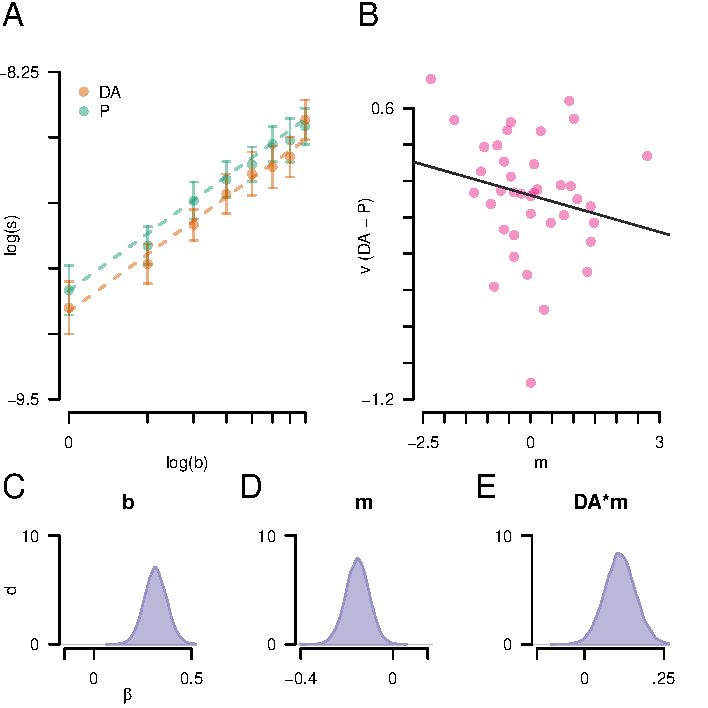
\includegraphics[width=0.7\linewidth]{../../images/s_fig} 

}

\caption{The influence of dopamine and mindfulness on door selection stereotypy. A) Accuracy (acc) data by block and drug. Circles reflect observed average variance (of the transition matrices), dotted lines show the fit of the winning model. B) The association between trait mindfulness (x-axis) and the impact of drug on variance [DA-P]. The bottom row shows posterior densities (in log odds) estimated for C) the main effect of block (b), D) the main effect of DA, and E) the drug x mindfulness (m) interaction. DA = dopamine, P = placebo, d = density. Error bars reflect within-subject standard error of the mean [SE].}\label{fig:stereofig}
\end{figure}

\bibliographystyle{unsrt}
\bibliography{references.bib}


\end{document}
